% arXiv preprint. Plain article class on purpose: no venue is claimed.
\documentclass[10pt,twocolumn,letterpaper]{article}

\usepackage[letterpaper,margin=1in,columnsep=20pt]{geometry}
\usepackage[T1]{fontenc}
\usepackage[utf8]{inputenc}
\usepackage{lmodern}
\usepackage{amsmath}
\usepackage{booktabs}
\usepackage{graphicx}
\usepackage{placeins}
\usepackage[round,authoryear]{natbib}
\usepackage{xcolor}
\definecolor{linknavy}{RGB}{0,51,153}
\usepackage[colorlinks=true,linkcolor=linknavy,citecolor=linknavy,urlcolor=linknavy,
            pdftitle={Only one arm's ceiling is estimable: engineered features versus learned sequence representations across 10k to 1.1M claims patients},pdfauthor={Daniel Gabra, Cyril Rakovski}]{hyperref}

% Stock float parameters push two-column floats pages away from the text that calls them.
\setcounter{topnumber}{4}
\setcounter{totalnumber}{6}
\renewcommand{\topfraction}{0.95}
\renewcommand{\textfraction}{0.05}
\renewcommand{\floatpagefraction}{0.75}

\bibliographystyle{plainnat}

\title{\bfseries Only one arm's ceiling is estimable: engineered features versus learned sequence representations across 10k to 1.1M claims patients}
\author{\textbf{Daniel Gabra, Cyril Rakovski}\\[3pt]{\normalsize \emph{Schmid College of Science and Technology, Chapman University}}}
\date{}

\begin{document}
\maketitle
\begin{abstract}

Whether learned representations of clinical event sequences can displace hand-engineered features
is usually settled in the few-shot regime, where count-based features hold their own. \textbf{Our
contribution is an evaluation design for asking that question at scale, and the result below is
its first application:} a pre-registered information-matching contract fixing what each arm may
see, a nested ladder spanning two orders of magnitude, identifiability-aware curve fitting that
reports ``not identifiable'' as a substantive outcome, and five ablations each targeting one named
alternative explanation.

Using a 1.25M-patient extraction from a national US commercial claims database, we predict
new-onset arthritis in the 12 months after a 12-month observation window, comparing 828
engineered features with gradient-boosted trees, a Deepr-style 1-D CNN and a BEHRT-style
Transformer over identical tokens, across a 10k to 1.11M ladder against one fixed 2023 holdout of
137,689 patients (1.85\% incident).

Engineered features lead at every scale; at 1.11M the gap to the Transformer is 0.0216 AUROC (95\%
CI 0.0183 to 0.0247). The informative result is shape rather than ranking: only the feature arm's
asymptote is identifiable across fit windows, placing it within 0.001 to 0.010 AUROC of its
ceiling, while neither sequence arm's is determined by data of this size. Under log-linear gap
closure, parity arrives near \textbf{6 to 8 million patients}.

Of five ablations, four exclude an alternative explanation and one bounds it. \textbf{Increasing
Transformer capacity is significantly harmful at the largest rung} (-0.0050 AUROC, CI -0.0073 to
-0.0030), opposite to the field's default intuition, and quadrupling the training budget changes
nothing, refuting our own earlier reading that the sequence arms were optimisation-limited.
Context length is the exception: it closes 15\% of the gap, but 14.1\% of cases remain truncated,
so we bound rather than exclude it. What remains is \textbf{data}.

\end{abstract}





\section*{Data and code availability}



The IQVIA PharMetrics Plus extraction \textbf{cannot be shared}: it is commercially licensed and redistribution is prohibited. Researchers with their own licence can reproduce the cohort exactly, since the extraction SQL, phenotype definition, eligibility criteria and vocabulary construction are released with the code. The full pipeline is released, with per-run configurations and metrics for all 234 training runs, per-rung AUROC and AUPRC at all six rungs, seed standard deviations, paired intervals for every arm pair, and the operating-point table at every alert budget. Code is available from the authors on request. Per-patient test predictions, used for every confidence interval reported here, are retained but not released, being keyed to identifiers from the licensed extraction.



\section{Introduction}\label{sec:1}



Claims and EHR data arrive as ordered sequences of coded events, which invites sequence models: recurrent networks, convolutional encoders, and more recently transformers pretrained on patient timelines. The competing tradition aggregates the same events into counts and hands them to gradient-boosted trees. Recent careful comparisons favour the count-based approach: on the EHRSHOT benchmark (6,739 patients, few-shot tasks), \citet{gao2025countbased} find head-to-head wins split largely between count-based learners and a mixture-of-agents LLM pipeline, with a pretrained transformer as a third comparator.



The obvious objection is that these are few-shot evaluations, and label scarcity is not where a supervised sequence model is supposed to win. That objection is rarely tested, because assembling two or three orders of magnitude more \textbf{labelled} patients for a single outcome is difficult. This paper tests it, and finds that the answer does not change.



\textbf{Our primary contribution is an evaluation design, and the arthritis result is its first application.} Representation comparisons in this literature are usually reported as a table of numbers with the two arms built under different constraints, which makes a loss hard to attribute: to the representation, or to whichever arm was fed less. We therefore specify the comparison before running it, and report where our own specification failed.



\begin{enumerate}
\item \textbf{An information-matching contract}, pre-registered: the same claims from the same window, the same frozen vocabulary chosen label-free, the same treatment exclusions, validation carve and test set. Section~\ref{sec:3.1} quantifies the three asymmetries that survived it, in both directions, rather than asserting the arms were matched.
\item \textbf{A scale-resolved ladder}: nested subsets from 10k to 1.11M, identical across arms and seeds, with one fixed temporal holdout, turning ``which representation wins'' into the answerable ``at what scale, if ever''.
\item \textbf{Identifiability-aware curve fitting}: we fit under multiple windows and report \textbf{``not identifiable'' as a substantive result} rather than presenting whichever fit converged.
\item \textbf{An elimination structure}: five ablations, each targeting one named alternative explanation, with paired bootstrap intervals. One refuted a claim we made earlier, and we report that reversal.
\end{enumerate}



Applying it gives: engineered features lead at every measured scale; only the feature arm's approach to saturation is estimable from this range; parity under log-linear closure arrives near 6 to 8 million patients; and increasing Transformer capacity is significantly \emph{harmful} at the largest rung. Section~\ref{sec:6} is explicit that this is not the same as out-scaling a \emph{pretrained} sequence model, which has typically seen more patient data than we use here.







\section{Data and cohort}\label{sec:2}



\textbf{Source.} One extraction from IQVIA PharMetrics Plus, de-identified US commercial medical and pharmacy claims: a 20\% hash sample of patients with at least 24 months of continuous enrollment, giving 2,017,387 patients and 1.28 billion month-granular claim rows spanning 201901 to 202412.



\textbf{Task.} For each patient the index month is the 13th month of their first qualifying enrollment span. The \textbf{observation window} is the 12 months before index, and every feature and token comes only from that window. The \textbf{outcome} is incident arthritis in the 12 months from index, defined as at least two distinct calendar months carrying a qualifying diagnosis (ICD-10 M05 to M08, M10, M12, M13, M15 to M19, M45, L40.5). Patients with any qualifying diagnosis before index are excluded as prevalent, so the label is new onset among patients who appear disease-free. Eligibility requires age 18 to 89 at index and 24 months of continuous enrollment, so a negative label reflects observed absence rather than disenrollment.



\textbf{Cohort.} 1,251,833 patients, 23,934 incident cases (1.91\%).



\textbf{Temporal validation.} Index years 2020 to 2022 form the training pool (1,114,144 patients); index year 2023 is a held-out test set (137,689 patients, 2,554 cases, 1.85\%) used once per run, never for model selection.



\subsection{Why this prediction problem matters clinically}\label{sec:2.1}



Most incident arthritis is diagnosed only once a patient presents with established symptoms. A claims-based onset model is not a diagnostic but a triage signal for deciding whom to surface for earlier assessment, so the relevant question is what an operating point buys. On our held-out year, flagging the highest-risk 5\% of patients (6,884 of 137,689) captures 743 of 2,554 incident cases: 29.1\% of cases at 10.8\% precision, a 5.8-fold enrichment over the 1.85\% base rate, or roughly nine patients reviewed per case found. At the top 1\% the enrichment is 8.6-fold.



The choice also has practical stakes: a sequence model costs substantially more to train, serve and re-validate than counts feeding a tree ensemble, so establishing which representation wins at realistically assemblable scale is directly actionable. We make no deployment claim; prospective validation, calibration and subgroup fairness analysis are each prerequisites and none is attempted here.



\subsection{Two properties of this cohort that constrain interpretation}\label{sec:2.2}



\textbf{Enrollment left-truncation.} Enrollment data begins at 201901, so patients already enrolled when the window opens all receive a first month of 201901: 597,065 patients, 47.7\% of the cohort, all falling in index year 2020, which is 61.9\% of the training pool. The 2023 test set contains none of them, so training and test differ in enrollment tenure as well as time, region mix shifts by up to 7.0 points, and the index-2020 stratum's outcome window overlaps the 2020 care disruption. Appendix A tests whether this drives the arm ranking; it does not. Because ladder subsets are drawn uniformly at random from the training pool, this composition is constant across rungs, so the \emph{shape} of the curves is unaffected even though the \emph{levels} are.



\textbf{Observation-window sparsity.} 15.7\% of non-cases and 3.3\% of cases have no claims at all in the observation window and are retained with demographics only.







\section{Three representations under an information-matching protocol}\label{sec:3}



The comparison is only meaningful if the arms differ in representation rather than in the information they see, so we fixed that contract before running any model.



\textbf{Shared across arms.} The same observation window, cohort, nested training subsets at 10k / 30k / 100k / 300k / 1M / 1,114,144, three seeds, the same 10\% training-carved validation split and the same fixed test set. Vocabularies are chosen label-free from the training pool by patient frequency, frozen, and applied identically to every rung and to the test set; phenotype codes cannot enter. Disease-specific treatments (DMARDs, biologics, urate-lowering agents) are excluded while symptomatic analgesics are retained, because the former encode uncoded disease and the latter are legitimate pre-symptomatic signal.



\textbf{The arms.} Arm A is 828 order-free engineered features with gradient-boosted trees, spanning demographics, comorbidity flags, utilisation counts, recency, a 500-category bag of 3-character ICD-10 codes, 96 therapeutic-class counts and a 200-code procedure bag. Arm B is a Deepr-style 1-D CNN over the same claims as an ordered token sequence, using Arm A's frozen vocabulary (798 tokens) plus the same seven demographics, truncated to the most recent 200 tokens. Arm C is a BEHRT-style Transformer encoder over identical tokens and demographics, \textbf{410,497 parameters}.



Each arm runs one fixed configuration with no per-size or per-seed search (hyperparameters in Appendix B); section~\ref{sec:5.3} shows this parity rule is not doing hidden work.



\subsection{Where the protocol is imperfect}\label{sec:3.1}



Three asymmetries survived, and we quantify rather than deny them. \textbf{Context truncation favours Arm A}: sequences are capped at 200 tokens while Arm A aggregates the window uncapped, truncating 40.1\% of incident cases against 17.2\% of non-cases, so the sequence arms see a censored view of the class that determines AUPRC (section~\ref{sec:5.1} measures the consequence). \textbf{Out-of-vocabulary handling favours Arms B and C}: codes outside the frozen vocabulary are dropped by Arm A but keep a positional UNK placeholder in the sequence arms, affecting 7.2\% of diagnosis and 35.8\% of procedure rows. \textbf{Order granularity limits what the contrast can mean}: claims are month granular and within-month order is arbitrary, so the only information the sequence arms hold that Arm A lacks is which of 12 months an event fell in (section~\ref{sec:5.4}).







\section{Results}\label{sec:4}



\subsection{Learning curves}\label{sec:4.1}





\begin{figure*}[t]

\centering

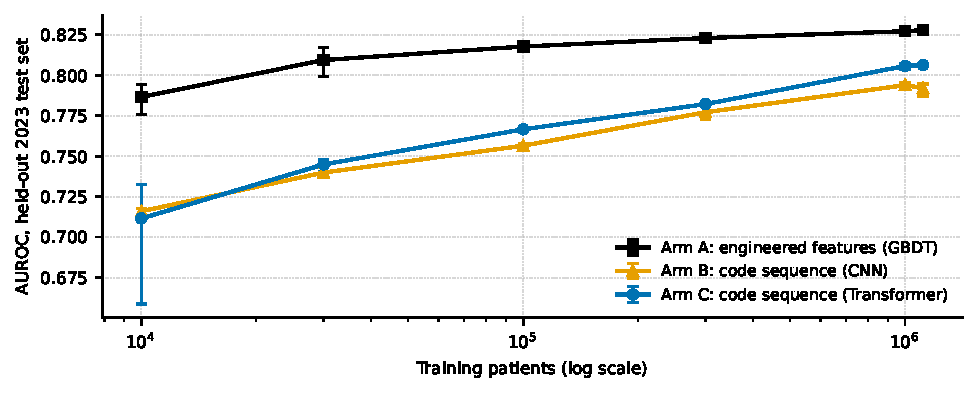
\includegraphics[width=0.74\textwidth]{fig1_learning_curves.pdf}

\caption{\textbf{Learning curves across the ladder.} AUROC on the fixed 2023 holdout against training-set size. Engineered features lead at every rung. Bars show the range over seeds, which is training variability rather than the sampling error of the metric; section~\ref{sec:4.2} gives the paired intervals that quantify the differences. The wide Arm C bar at 10k is the training instability documented below.}

\end{figure*}



\begin{table*}[tbp]
\centering
\small
\caption{AUROC on the fixed 2023 holdout, mean over seeds (SD in brackets).}
\label{tab:1}
\begin{tabular}{llll}
\toprule
training patients & A features & B CNN & C Transformer \\
\midrule
10,000 & 0.7865 (0.0098) & 0.7160 (0.0033) & 0.7115 (0.0302) \\
100,000 & 0.8177 (0.0011) & 0.7565 (0.0009) & 0.7666 (0.0006) \\
1,114,144 & \textbf{0.8279} (0.0005) & 0.7920 (0.0042) & 0.8063 (0.0006) \\
\bottomrule
\end{tabular}
\end{table*}



Table~\ref{tab:1} gives AUROC on the fixed 2023 holdout at three rungs, with the seed-to-seed standard deviation in brackets. Seeds are three per cell throughout, except \textbf{Arm C at 10,000, which uses five} (see the corrected-configuration note below).



AUPRC at the same rungs: A rises 0.0601 to 0.0891, B 0.0416 to 0.0702, C 0.0407 to 0.0775 against a base rate of 0.0185, so the feature arm averages roughly 4.8 times the base rate across the precision-recall curve. That is a curve-wide average, not the 5.8-fold enrichment quoted at the top-5\% operating point in section~\ref{sec:2.1}.



\textbf{The 10k rung uses a corrected Arm C configuration.} Under the frozen configuration Arm C failed to train at 10k: two of three seeds stopped at the first epoch, seed SD 0.0900 against 0.0006 at the top rung. Re-running with warmup 100, patience 10 and five seeds recovered +0.095 AUROC and cut the spread to 0.0302. We report the corrected value and disclose that it mixes configurations across the ladder; section~\ref{sec:5.3} shows schedule settings are inert at every rung where training succeeds.



\textbf{The Transformer does not dominate the older CNN at every scale.} At 10k the CNN retains a small but detectable edge (-0.0045, 95\% CI -0.0085 to -0.0003); the Transformer leads from 30k, reaching +0.0143 at the top rung. A top-rung-only comparison would hide that.



\textbf{Feature-set ablations within Arm A.} The 27-feature \texttt{thin} set reaches 0.8239 AUROC at the top rung, so bag-of-codes enrichment is worth +0.0040. Stripping every utilisation and recency feature costs +0.0023; at 0.8256 that access-stripped arm still leads the Transformer's 0.8063, so the headline gap is not an access artefact.



\subsection{Uncertainty, reported correctly}\label{sec:4.2}



Standard deviation over training seeds is not the sampling error of the metric. At the top rung Arm A's AUROC has a DeLong standard error of \textbf{0.0036} on 2,554 cases, while its seed-to-seed spread is \textbf{0.0005}, roughly sevenfold smaller; reporting the latter as an error bar would overstate precision by an order of magnitude.



Because every run persists per-patient test predictions, arms are compared \textbf{paired on the same patients}, which is both correct and far tighter than differencing two independent estimates. Intervals come from 2,000 bootstrap resamples stratified to preserve the case count, each arm's value being the seed-mean of the per-seed metric so the intervals attach to the numbers in section~\ref{sec:4.1}.



\begin{table*}[tbp]
\centering
\small
\caption{AUROC gaps with 95\% CI.}
\label{tab:2}
\begin{tabular}{llll}
\toprule
training patients & A - C & A - B & C - B \\
\midrule
10,000 & +0.0750 [+0.0683, +0.0815] & +0.0705 [+0.0637, +0.0773] & -0.0045 [-0.0085, -0.0003] \\
100,000 & +0.0511 [+0.0454, +0.0568] & +0.0612 [+0.0553, +0.0670] & +0.0101 [+0.0069, +0.0135] \\
1,114,144 & \textbf{+0.0216 [+0.0183, +0.0247]} & +0.0358 [+0.0315, +0.0402] & +0.0143 [+0.0113, +0.0172] \\
\bottomrule
\end{tabular}
\end{table*}



Table~\ref{tab:2} gives the paired AUROC gaps between every pair of arms, with 95\% intervals. AUPRC at the top rung: A - C = +0.0116 [+0.0070, +0.0164]. Every AUROC comparison at every rung excludes zero.



Ensembling three seeds narrows the gaps (A - C +0.0216 to +0.0158, A - B +0.0358 to +0.0277), so part of the deficit is variance rather than bias. Single-model numbers are primary, being what the curves and fits use.



\subsection{The shape result}\label{sec:4.3}



Fitting a saturating power law, $\mathrm{AUROC}(n) = c - a n^{-b}$, per arm and fit window (full table in Appendix D), Arm A yields a ceiling of \textbf{0.8292} over all rungs and \textbf{0.8379} excluding 10k, leaving it \textbf{0.0014 to 0.0100} below its own asymptote. Neither sequence arm yields a ceiling under both windows: each is identifiable only with the least stable rung included, returning 0.913 for the CNN and 0.891 for the Transformer, with 0.12 and 0.08 of headroom from curves that moved only 0.076 and 0.095 across two decades. This is substantive rather than a convergence failure: the unconstrained fit pushes the asymptote against the AUROC bound with the exponent pinned at the grid edge, so the range cannot distinguish a high ceiling approached slowly from a lower one reached later.



\textbf{The defensible claim} is that the engineered-feature arm is the only one whose approach to saturation is estimable across both windows, every estimate placing it within 0.01 AUROC of its ceiling. \textbf{This is an asymmetry in what we can estimate, not in what has happened}: the ambiguity includes a sequence arm being \emph{nearer} its ceiling than its slope suggests, so we do not claim they failed to saturate.



\subsection{Where parity would occur}\label{sec:4.4}





\begin{figure*}[t]

\centering

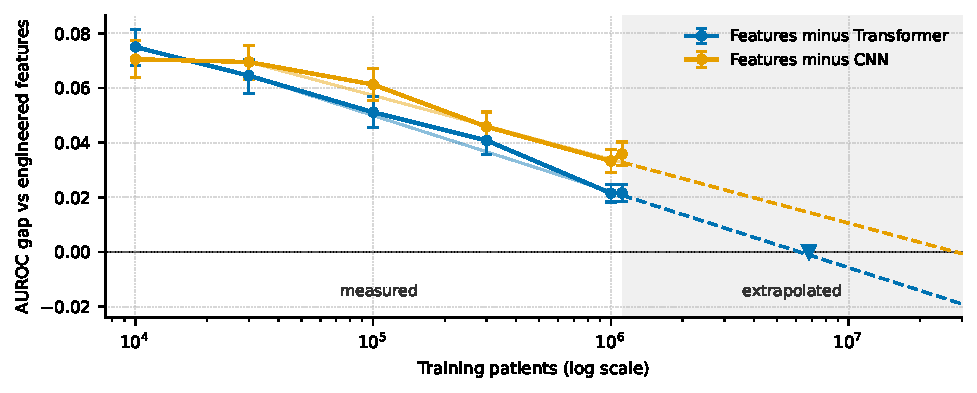
\includegraphics[width=0.74\textwidth]{fig2_gap_closure.pdf}

\caption{\textbf{Gap closure and extrapolated parity.} The AUROC gap between engineered features and each sequence arm, with paired bootstrap 95\% intervals. The shaded region is extrapolated rather than measured; the fitted lines there assume log-linear closure and exclude the 10k rung, and the triangle marks extrapolated parity for the Transformer. The extrapolation is an assumption about what happens beyond our data, not a measurement.}

\end{figure*}



Fitting the arm gap against $\log_{10} n$ (full table in Appendix D), the features-versus-Transformer gap closes at -0.0265 per decade over all rungs, -0.0279 excluding 10k and -0.0296 from 100k upward, placing extrapolated parity at 7.8e6, 6.8e6 and 5.9e6.



\textbf{Under log-linear gap closure, engineered features and a from-scratch Transformer reach parity at roughly 6 to 8 million training patients}, five to seven times our largest rung. The estimate varies only 1.3-fold across fit windows, so unlike the corresponding CNN figure (3.1-fold) it is stable enough to quote as an estimate rather than a bound.



That stability follows from correcting the 10k rung: with the failed runs in place the all-rungs fit returned 1.6e6 and the spread was 4.2-fold. Since the estimate rests on that correction, we checked the corrected configuration is not simply more favourable: re-running Arm C at 30k and 100k under it moves AUROC by +0.0020 and +0.0008.







\section{Does the result survive our own design choices?}\label{sec:5}



Five choices could produce this result artefactually. We tested all five, four here and the enrollment-boundary stratum in Appendix A; section~\ref{sec:5.5} states what that leaves.



\subsection{Context length}\label{sec:5.1}



A 512-token window reduces case truncation from 40.1\% to 14.1\% and non-case truncation from 17.2\% to 4.7\%, removing roughly two thirds of the differential censoring. The Transformer gains \textbf{+0.0045 AUROC} (95\% CI +0.0017 to +0.0072) at 300k and +0.0032 (+0.0003 to +0.0061) at the top rung on a single-seed spot check; the CNN gains +0.0011 at 300k, not distinguishable from zero.



Longer context genuinely helps the Transformer, and helps AUPRC proportionally more than AUROC, the signature predicted if the binding problem was censoring of the positive class: at the top rung it closes \textbf{15\% of the AUROC gap and 35\% of the AUPRC gap}. The asymmetry was real and worth correcting, but does not explain the result.



\subsection{Model capacity}\label{sec:5.2}



Holding model size fixed while scaling data is the standard way to manufacture a plateau, so the claim requires evidence that capacity is not binding.



Doubling depth from the 410k-parameter headline model changes AUROC by \textbf{-0.0005} at 300k (95\% CI -0.0024 to +0.0014) and by \textbf{-0.0050 at the top rung} (-0.0073 to -0.0030), where the interval excludes zero in the negative direction. A wider model (d192/L4, 3.4x parameters) at 300k also fails to help: -0.0014 [-0.0039, +0.0010]. Extra capacity is neutral at 300k and \textbf{significantly negative at the top rung}, an interaction that runs opposite to what a capacity explanation requires, since more data makes extra depth less useful rather than more.



\subsection{Optimisation budget}\label{sec:5.3}



Our earlier reading was that the sequence arms were budget-limited: every run early-stopped between epochs 3 and 7 of an allowed 25, and seed ensembling helped. We tested that directly, and \textbf{it is wrong}.



Re-running with the epoch cap raised from 25 to 100, patience from 4 to 15 and cosine decay added, with Arm A given a matched extension from 800 to 2,400 rounds and patience 40 to 100: at the top rung no arm moves by more than 0.0014, and \textbf{the selected epoch is identical to the frozen-budget run} (267.7 rounds for Arm A, 3.0 epochs for Arm B, 6.3 for Arm C). Arm C stops at epoch 6 of 100 allowed; Arm A uses 268 of 2,400. The models are not budget-limited. The same insensitivity holds for the schedule's shape: re-running Arm C at 30k and 100k with the shorter warmup and longer patience used for the corrected 10k rung moves AUROC by +0.0020 and +0.0008. Arm C is insensitive to schedule settings at 30k, 100k, 300k and 1,114,144, and sensitive only at 10k, where the frozen configuration failed to train at all.



Seed ensembling nonetheless still narrows the gap by 0.0058 (section~\ref{sec:4.2}), so a share of the deficit is variance that a longer schedule does not reduce. The instability is in which solution a run converges to, not whether it has converged.



\subsection{Monthly temporal resolution (Arm A-M)}\label{sec:5.4}



The only information the sequence arms hold that the order-free bag lacks is which of the 12 observation months an event fell in (section~\ref{sec:3.1}). Arm A-M gives the bag exactly that: every count feature split into 12 monthly bins, 9,672 columns, same vocabulary, exclusions, untuned configuration, ladder, seeds and test set. If A-M closed the gap, our conclusion would concern temporal resolution rather than representation learning.



It does not. A-M is \textbf{significantly worse than Arm A at all six rungs}, by -0.0043 (95\% CI -0.0059 to -0.0027) at the top rung, where it still leads the Transformer by +0.0173 (+0.0139 to +0.0208). A-M's fitted ceiling sits below Arm A's and its gap-closure slope against Arm C is identical at -0.0279 per decade: binning shifts the level slightly and the shape not at all.



Because the sparse matrix is 99.2\% zero and XGBoost treats structural zeros as missing rather than zero, an aggregated control pooled back to Arm A's 828 columns, verified to reproduce its feature values exactly, tracks dense Arm A to -0.0004 [-0.0011, +0.0002] at the top rung. The sparse encoding is not driving the comparison.



\textbf{No binning of the bag beats Arm A, at any granularity.} At the top rung AUROC falls monotonically as the bag is split more finely: 0.8279 at 828 columns, 0.8261 at two 6-month bins, 0.8250 at four 3-month bins, 0.8236 at twelve. The penalty is a smooth dose-response rather than a cliff at the finest binning, and it is already significant at two bins (-0.0018, 95\% CI -0.0029 to -0.0006), which carry only twice Arm A's column count. On AUPRC the two coarse variants are indistinguishable from Arm A, so the claim is that binning costs ranking accuracy, not that it harms both metrics.



\textbf{Caveat.} Binning granularity and column count are confounded by construction, and A-M's 11.7x feature count sits under the same untuned \texttt{colsample\_bytree} of 0.8, so the claim is that temporal resolution does not help \textbf{under matched, untuned hyperparameters}, not that it cannot help.



\subsection{What these ablations do and do not exclude}\label{sec:5.5}



Four explanations are excluded outright: \textbf{capacity does not help} (section~\ref{sec:5.2}, and it hurts at the top rung), \textbf{a longer or differently shaped schedule does not help} (section~\ref{sec:5.3}), and \textbf{monthly temporal resolution does not help} (section~\ref{sec:5.4}, under matched untuned hyperparameters), and \textbf{the enrollment-boundary stratum does not drive the ranking} (Appendix A). One is bounded rather than excluded: \textbf{longer context does help} (section~\ref{sec:5.1}), and with 14.1\% of cases still truncated at 512 tokens we cannot rule out further gains. Its disproportionately larger AUPRC effect is the signature of positive-class censoring, so that mechanism is live rather than exhausted.



The dominant remaining constraint is therefore data: the sequence arms' position on their curves is not an artefact of capacity, optimisation or temporal binning.



\section{Related work}\label{sec:6}



Learning patient representations end to end runs from Deepr \citep{nguyen2017deepr}, the ancestor of our Arm B, through BEHRT \citep{li2020behrt} and Med-BERT \citep{rasmy2021medbert} to CLMBR \citep{steinberg2021clmbr}, while outside healthcare gradient-boosted trees on tabular features remain hard to beat \citep{shwartzziv2022tabular,grinsztajn2022trees}. The comparison is usually settled in the few-shot regime: on EHRSHOT \citep{wornow2023ehrshot}, \citet{gao2025countbased} report wins split largely between count-based learners and a mixture-of-agents LLM pipeline, with a pretrained transformer as a third comparator.



\textbf{We confirm rather than overturn that result, and add a scale dimension to it.} Their transformer is pretrained on 2.57M patients while ours are trained from scratch, so in patient data seen we sit below their setting; what we increase by two orders of magnitude is the labelled supervised training set, the axis their few-shot design holds small. From the scaling-law literature \citep{hestness2017scaling,rosenfeld2020constructive,kaplan2020scaling,hoffmann2022training} we take the saturating functional form and the warning that a scaling claim made while holding capacity fixed is not interpretable, which is why section~\ref{sec:5.2} reports a capacity-by-data interaction. Appendix C expands both threads.







\section{Limitations}\label{sec:7}



\textbf{No pretraining, and this is the most important limitation.} All arms are trained from scratch, while the sequence models this literature deploys are pretrained: the closest comparison work uses a 141M-parameter model pretrained on 2.57M patients, roughly 340x our parameter count and more patient data than our largest rung. Our result therefore bounds what a \emph{from-scratch} sequence model achieves with abundant labels and says nothing about a pretrained one. This is the most plausible route by which our conclusion fails, and our extraction is large enough to test it.



\textbf{Single population, single phenotype.} One commercial insurer, one outcome, no clinical adjudication. Arthritis across seven subtypes is clinically heterogeneous, and with prior joint and back pain among the features, part of what is predicted is a coding event in patients with existing musculoskeletal complaints.



\textbf{Temporal validation is confounded with an enrollment-cohort shift} (section~\ref{sec:2.2}). We show the scaling shape is unaffected, but do not disentangle it.



\textbf{Arm A lacks ontology structure.} Diagnoses enter as a flat 3-character bag where comparable count baselines use ontology roll-ups, so Arm A does not reproduce those baselines.



\textbf{Tuning parity is weaker than it looks.} Both arms run one fixed configuration, but robustness to being untuned is not symmetric between trees and transformers. Section~\ref{sec:5.3} partly addresses this; a matched validation search would be stronger.



\textbf{The parity estimate assumes log-linear gap closure}, and neither sequence arm has an asymptote identifiable across fit windows, so we cannot exclude their curves bending before parity. The 1.3-fold stability across windows bounds analysis-choice sensitivity, not the functional form.



\textbf{Two definitional gaps.} The 10k rung mixes configurations, for the reason given in section~\ref{sec:4.1}, and the phenotype regex omits M1A, M11 and M14, affecting 0.2\% of patients with a baseline diagnosis.







\section{Conclusion}\label{sec:8}



At 1.11 million labelled training patients, two orders of magnitude beyond the few-shot regime in which this comparison is usually made, hand-engineered claims features with gradient-boosted trees still outperform learned sequence representations trained from scratch, by 0.0216 AUROC (95\% CI 0.0183 to 0.0247). The more useful finding is that the families sit at different points on their curves: the feature arm's ceiling is estimable and lies within 0.01 AUROC of where it already is, while the sequence arms' asymptotes are not determined by data of this size, and under log-linear closure parity arrives near 6 to 8 million patients. What makes that defensible is what we could not explain it away with: section~\ref{sec:5} rules out capacity, training budget and temporal resolution, and Appendix A the enrollment-boundary stratum, leaving context length as the one lever that moves, bounded rather than eliminated.



For practitioners building risk models on claims at realistic scale, feature engineering remains the better investment. For method developers, a larger model and a longer schedule are both inert at this scale; the useful targets are a longer observation window and, above all, \textbf{pretraining}, which our from-scratch design does not test.







\section*{Ethics and data statement}



\textbf{Data and human subjects.} IQVIA PharMetrics Plus is a de-identified administrative claims database licensed to the authors' institution and containing no direct identifiers. This study is a secondary analysis of fully de-identified records.



\textbf{Compute.} All models trained on a single NVIDIA T4 or a 4-core laptop CPU, approximately 40 GPU-hours in total. No result here requires cluster-scale compute, which is deliberate: an evaluation design only a well-resourced group can run is not a useful contribution.







\section*{Acknowledgements}



This work was supported by the Chapman University Summer Undergraduate Research Fellowship (SURF), 2026.





\label{main:end}
\bibliography{refs}
\onecolumn\label{app:start}\appendix



Reviewers are not obligated to read supplementary material. Everything load-bearing for the argument is in the main text; what follows is supporting detail.



\section{The enrollment-boundary sensitivity analysis}



Section~\ref{sec:2.2} documents that 47.7\% of the cohort share an artificial 201901 first-enrollment month and that none of them are in the test set. We tested whether that drives the ranking by dropping index year 2020 entirely, reducing the training pool from 1,114,144 to 424,458 and removing all 597,065 boundary patients, against the same fixed 2023 test set.

\begin{table}[!ht]
\centering
\small
\label{tab:3}
\begin{tabular}{lll}
\toprule
rung & A - C, restricted & A - C, full pool \\
\midrule
30,000 & +0.0648 & +0.0645 \\
100,000 & +0.0450 & +0.0511 \\
300,000 & +0.0398 & +0.0408 \\
424,458 & +0.0381 & (beyond restricted pool) \\
\bottomrule
\end{tabular}
\end{table}



At matched training size the gaps are essentially unchanged. The confound affects the absolute level of every arm and is a real limitation of the cohort design, but it does not produce the arm ranking or the shape of the curves.







\section{Per-arm hyperparameters}



The three surviving information asymmetries, and their measured sizes, are stated in section~\ref{sec:3.1} and not repeated here.



\textbf{Arm A.} XGBoost, histogram method, max depth 6, learning rate 0.05, subsample 0.8, \texttt{colsample\_bytree} 0.8, minimum child weight 5, up to 800 boosting rounds with early stopping at 40 on validation AUC, no positive-class reweighting. 828 features. Two reduced sets are also reported: \texttt{thin} (27 features) and \texttt{rich\_noutil} (815, dropping every utilisation and recency feature).



\textbf{Arm B.} Embedding dimension 64 with learned positional encoding, multi-kernel 1-D convolution with kernels \{3, 5\} and 64 filters each, masked global max-pooling, MLP head of width 64, dropout 0.2. Adam, learning rate 1e-3, batch 512, up to 25 epochs, patience 4 on validation AUROC.



\textbf{Arm C.} d\_model 128, 8 attention heads, 2 layers, feed-forward width 256, dropout 0.2, GELU, pre-norm, a learnable CLS token with learned positional embeddings, CLS pooling, MLP head. AdamW, learning rate 3e-4, weight decay 1e-2, 300-step linear warmup, gradient clipping 1.0, batch 512, up to 25 epochs, patience 4. \textbf{410,497 parameters.}



Neither arm receives a per-size or per-seed hyperparameter search. Section~\ref{sec:5.3} shows that extending the budget fourfold changes no arm's result and leaves the selected epoch identical.



\section{Extended related work}



\textbf{Sequence models for structured EHR.} Representing a patient as an ordered sequence of coded events and learning the representation end to end has a long line of work. Deepr \citep{nguyen2017deepr} applies a convolutional network over code sequences and is the direct ancestor of our Arm B. BEHRT \citep{li2020behrt} and Med-BERT \citep{rasmy2021medbert} adapt masked-language-model transformers to diagnosis sequences, and CLMBR \citep{steinberg2021clmbr} uses an autoregressive objective to produce reusable patient representations. Our Arm C follows the BEHRT design, with the important difference noted below that it is trained from scratch rather than pretrained.



\textbf{Count and tabular baselines.} In parallel, work outside healthcare has repeatedly found that gradient-boosted trees on tabular features remain hard to beat \citep{shwartzziv2022tabular,grinsztajn2022trees}, with the advantage attributed to robustness to uninformative features and to irregular target functions. Applied to claims and EHR, this argues for aggregating events into counts and letting a tree model do the selection, which is our Arm A.



\textbf{The comparison at small n.} EHRSHOT \citep{wornow2023ehrshot} provides 6,739 patients from Stanford Medicine and 15 few-shot tasks, explicitly designed to evaluate pretrained models under label scarcity. \citet{gao2025countbased} benchmark on it and report that head-to-head wins across eight tasks are largely split between count-based learners (LightGBM and TabPFN, built from \textbf{ontology roll-ups with two time bins}) and a mixture-of-agents LLM pipeline, with the pretrained transformer CLMBR as a third comparator. Their headline is that count-based approaches remain strong, not that transformers uniformly lose.



\textbf{Our relation to that work is narrower than it may appear, and we state it precisely.}



\begin{enumerate}
\item \emph{We do not run their comparison at larger scale.} CLMBR-T-base is a 141M-parameter model pretrained on 2.57M patients; EHRSHOT's 6,739 patients are the evaluation cohort, not the data the model has seen. Our sequence arms are 410k parameters trained from scratch. In terms of patient data seen by the sequence model, we are \textbf{below} their setting, not 100x above it. What we increase by roughly two orders of magnitude is the \textbf{labelled supervised training set for a single task}, which is the axis their few-shot design deliberately holds small.
\item \emph{Our engineered arm is structurally weaker than theirs.} Arm A uses a flat 3-character ICD-10 bag over one 12-month window with five light recency features, without ontology roll-ups and without their two time bins. That our weaker feature arm still leads is consistent with their conclusion, but Arm A should not be read as a reproduction of their baseline, and section~\ref{sec:7} treats the missing hierarchy and temporal resolution as a limitation rather than a design choice.
\item \emph{We therefore confirm rather than overturn the small-n finding, and add a scale dimension to it.} Our contribution is the evaluation design of section~\ref{sec:1}: the information-matching contract, the scale-resolved ladder, identifiability-aware fitting, and the elimination structure. The arthritis findings are what that design produced on its first application, not the contribution in themselves.
\end{enumerate}



\textbf{Scaling laws.} The empirical observation that error falls as a power law in data and model size, with a task-dependent irreducible term, was established by \citet{hestness2017scaling} and \citet{rosenfeld2020constructive} and made central by \citet{kaplan2020scaling} and \citet{hoffmann2022training}. We borrow the saturating functional form and, more importantly, the methodological warning: a scaling claim made while holding model capacity fixed is not interpretable, because a capacity-bound model plateaus for reasons unrelated to data. Section~\ref{sec:5.2} is a direct response to that warning, and it is why we report the capacity-by-data interaction rather than only the learning curves. Comparable scale-resolved analyses are uncommon in clinical prediction, where cohorts large enough to span three orders of magnitude for a single outcome are rare.



\section{Power-law and gap-closure fits}



\begin{table}[!ht]
\centering
\small
\caption{Saturating power law, $\mathrm{AUROC}(n) = c - a\,n^{-b}$, per arm and fit window.}
\label{tab:4}
\begin{tabular}{llllll}
\toprule
arm & fit window & ceiling c & exponent b & at top rung & headroom \\
\midrule
A features & all rungs & 0.8292 & 0.620 & 0.8279 & \textbf{+0.0014} \\
A features & excluding 10k & 0.8379 & 0.283 & 0.8279 & \textbf{+0.0100} \\
B CNN & all rungs & 0.9131 & 0.106 & 0.7920 & +0.1211 \\
B CNN & excluding 10k & not identifiable &  & 0.7920 &  \\
C Transformer & all rungs & 0.8906 & 0.156 & 0.8063 & +0.0843 \\
C Transformer & excluding 10k & not identifiable &  & 0.8063 &  \\
\bottomrule
\end{tabular}
\end{table}



\begin{table}[!ht]
\centering
\small
\caption{Gap closure against $\log_{10} n$, with the extrapolated parity point.}
\label{tab:5}
\begin{tabular}{llll}
\toprule
comparison & fit window & slope per decade & extrapolated parity \\
\midrule
A vs C & all rungs & -0.0265 & 7.8e6 \\
A vs C & excluding 10k & -0.0279 & 6.8e6 \\
A vs C & \textgreater{}= 100k & -0.0296 & 5.9e6 \\
\bottomrule
\end{tabular}
\end{table}



\begin{table}[!ht]
\centering
\small
\caption{Context-length ablations in full.}
\label{tab:6}
\begin{tabular}{llll}
\toprule
ablation & setting & AUROC delta [95\% CI] & AUPRC delta [95\% CI] \\
\midrule
512 vs 200 & Transformer, 300k & +0.0045 [+0.0017, +0.0072] & +0.0042 [+0.0013, +0.0073] \\
512 vs 200 & Transformer, top rung & +0.0032 [+0.0003, +0.0061] & +0.0041 [+0.0002, +0.0082] \\
512 vs 200 & CNN, 300k & +0.0011 [-0.0016, +0.0036] & +0.0029 [+0.0003, +0.0059] \\
\bottomrule
\end{tabular}
\end{table}



\begin{table}[!ht]
\centering
\small
\caption{Capacity ablation, doubling depth at fixed width.}
\label{tab:7}
\begin{tabular}{llll}
\toprule
rung & d128/L2 (410k params) & d128/L4 & delta [95\% CI] \\
\midrule
300,000 & 0.7822 & 0.7817 & -0.0005 [-0.0024, +0.0014] \\
1,114,144 & 0.8063 & 0.8012 & \textbf{-0.0050 [-0.0073, -0.0030]} \\
\bottomrule
\end{tabular}
\end{table}



\begin{table}[!ht]
\centering
\small
\caption{Longer-schedule results at the two largest rungs. Arm B at 300k is the only cell where the extended budget selects a different epoch, and it moves AUROC by -0.0014.}
\label{tab:8}
\begin{tabular}{llllllll}
\toprule
arm & rung & frozen budget & extended budget & delta & best epoch, frozen & best epoch, extended & cap \\
\midrule
A & 300,000 & 0.8230 & 0.8230 & +0.0000 & 137.0 & 137.0 & 2,400 \\
B & 300,000 & 0.7772 & 0.7758 & -0.0014 & 1.7 & 2.7 & 100 \\
C & 300,000 & 0.7822 & 0.7821 & -0.0000 & 3.7 & 3.7 & 100 \\
A & 1,114,144 & 0.8279 & 0.8279 & +0.0000 & 267.7 & 267.7 & 2,400 \\
B & 1,114,144 & 0.7920 & 0.7929 & +0.0009 & 3.0 & 3.0 & 100 \\
C & 1,114,144 & 0.8063 & 0.8064 & +0.0001 & 6.3 & 6.3 & 100 \\
\bottomrule
\end{tabular}
\end{table}



\end{document}
